\chapter{Processing the Captured Data}
This chapter is dedicated to the complex process of extracting critical data from the video files and IMU csv. 

\section{Processing the IMU Data}
The following flowcharts depicts the procedural processing of IMU data.
\begin{figure}[!ht]
  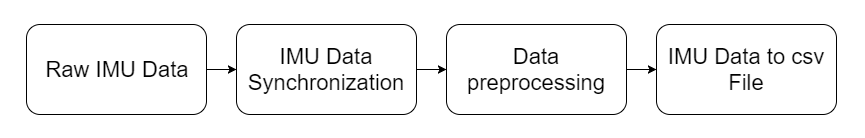
\includegraphics[width=\linewidth]{figures/imuflow.png}
  \caption{Diagram showing the progression and dependence of the major stages of video processing in the project}
  \label{fig:imuflow}
\end{figure}

\subsection{Obtaining IMU Data}
To use the smartphone as an IMU a free application "AndroSensor" \cite{androsensor} was installed. This application could log parameter from all the  sensor s and could be configured in various ways

\begin{figure}[!ht] 
\captionsetup{width=\linewidth, font=small}  
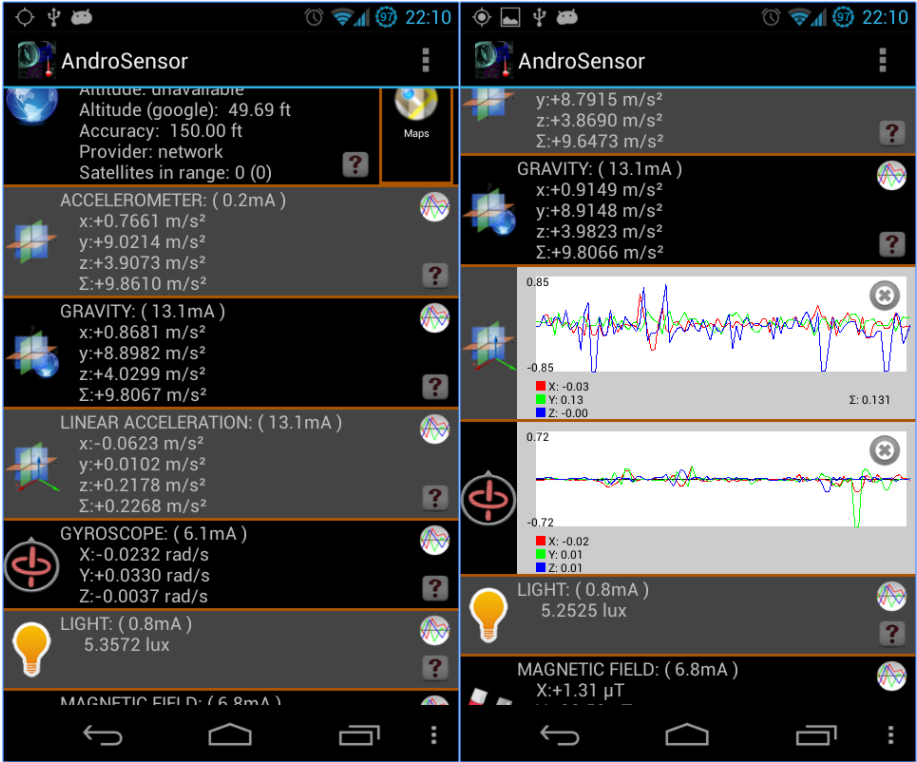
\includegraphics[width=\linewidth]{figures/as.png}
\caption{Androsensor Screenshots from \cite{androsensor}}
\label{fig:as}
\end{figure}

The IMU data logged by the smartphone was saved as a .CSV file with the first row containing the headings of various variables. These headings were

\begin{table}
\centering
\caption{This table shows the different headings of the output IMU file}
\label{IMU Headings}
\begin{tabular}{ll}
Heading               & Fields  \\
ACCELEROMETER       & X,Y,Z  \\
GRAVITY              & X,Y,Z \\
LINEAR ACCELERATION  & X,Y,Z\\
GYROSCOPE            & X,Y,Z \\
MAGNETIC FIELD       &  X,Y,Z\\
ORIENTATION          &  X,Y,Z\\
ATMOSPHERIC PRESSURE  &  \\
LOCATION Latitude     &  \\
LOCATION Longitude    &  \\
LOCATION Speed        &  \\
LOCATION ORIENTATION  & 
\end{tabular}
\end{table}

All these variables have been recorded with respect the smartphone frame of reference as shown below
\begin{figure}[!ht] 
\captionsetup{width=\linewidth, font=small}  
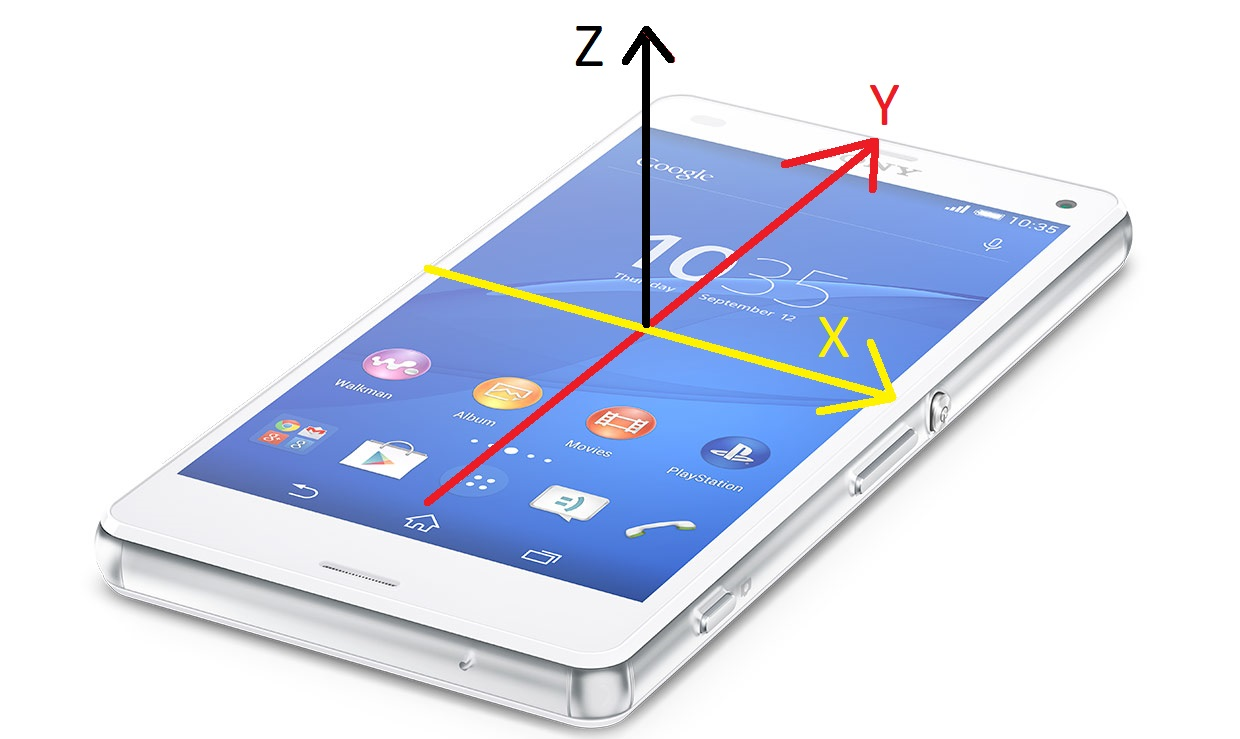
\includegraphics[width=\linewidth]{figures/phone.jpg}
\caption{Figure demonstrating the frame of reference of the smartphone}
\label{fig:phone}
\end{figure}

\subsection{Synchronizing IMU Data}

\subsection{Preprocessing IMU Data}
Before we can apply the IMU data directly to the EKF we need to make some minor modifications to the data. This is critical in removing any bias from the sensors. MEMS inherently have some 

\subsection{Exporting IMU Data}


\section{Processing the Video Data}
The following digram shows the process of converting a data heavy video file to a more lightweight .csv (Comma Separated Values) file.
\begin{figure}[!ht]
  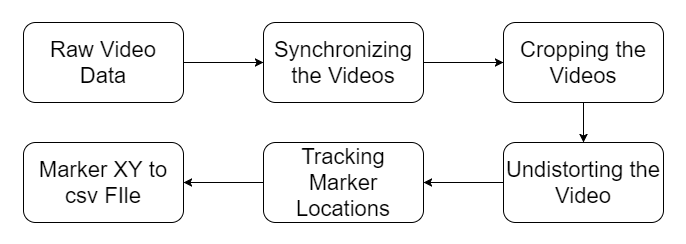
\includegraphics[width=\linewidth]{figures/videoProcess.png}
  \caption{Diagram showing the progression and dependence of the major stages of video processing in the project}
  \label{fig:videoProcess}
\end{figure}

\subsection{Obtaining Video Data}
Using the chest mounted cameras detailed in the previous chapter we can generate raw video data. The GPHS cameras can be configured to record at different frame rates and resolutions as discussed in the previous chapter. The video files where stored in an .MP4 format. This meant that during recording the video was compressed and the 


\subsection{Synchronizing Video Sources}
I typical problem faced when working with different sources of data is that of synchronization. Since this project used 4 different cameras, synchronizing the video sources are critical to generate accurate stereo vision data.

The problem of synchronization was overcome by using a audio cue to align the video data post capturing. With all systems recording, a simple hand clap can serve as a spiking audio input easily identified in the audio track of the video streams. The frame associated with this audio spike can be identified using SVP (Sony Vegas Pro) video editing software as shown in the figure below. 

\begin{figure}[!ht]
\centering
  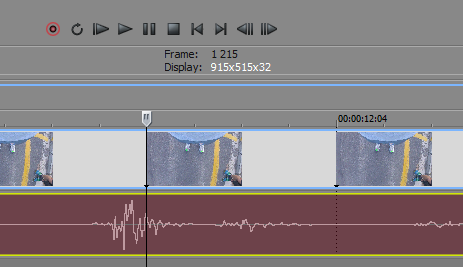
\includegraphics[width=0.5\linewidth]{figures/svpframe.png}
  \caption{Figure showing the user interface of SVP video editing software}
  \label{fig:svpframe}
\end{figure}

The red track in the above figure shows the recorded audio stream while the corresponding frames are displayed in the blue track above that. The cursor is aligned with the audio spike caused by the clap with the corresponding frame number displayed below the playback controls.

This method was repeated for every video stream such that a common starting point was generated. 

\subsection{Cutting Critical Video Data}
With the video data synchronized the next step was to generate a subset of video demonstrating a transient period and steady state period of running. From accelerometer readings we can easily determine the gait cycle period of our subject; that is the amount of time take between the same foot impacting the ground. These impacts are visible as spikes as seen in the accelerometer data.  

\subsection{Undistorting the Video Data}
To generate accurate distances using stereo vision the video frames need to be undistorted.

Distortion of the frames is a result of the 

To gain further understanding of undistorting video files \cite{Hartley2004} served as a reference. In this work Hartley describes various methods of undistorted images. These distortions are due to various lens effects.

\subsection{Tracking and Exporting Marker Positions in the Frame}

This section discusses the different methods of feature detection subdividing them into two main methodologies: automated and semi-automated. Each of these approaches offer advantages and disadvantages. To understand the approaches considered for this work it is important to visualize the input image data to the system. The following picture shows the various frames from all the cameras.

\begin{figure}[!ht]
  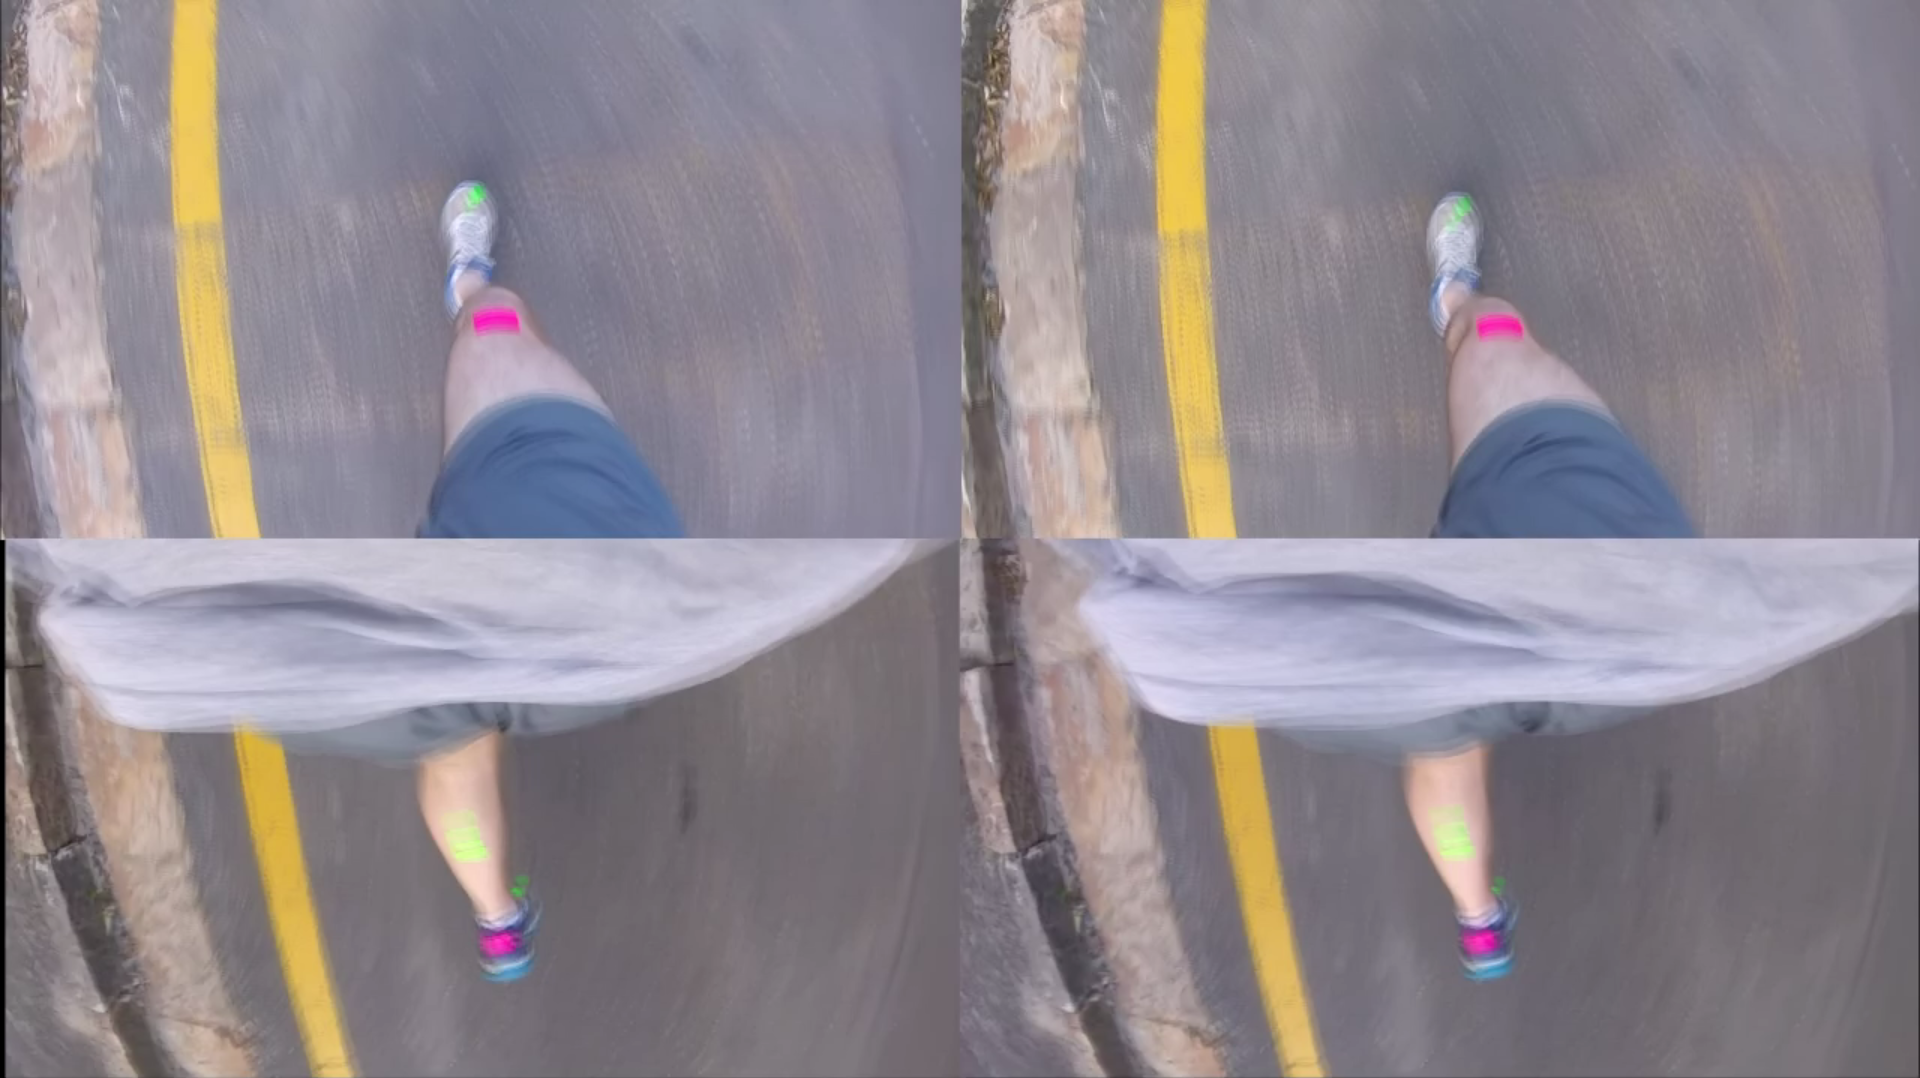
\includegraphics[width=\linewidth]{figures/pat_run_quad.png}
  \caption{4 Frames from the different cameras combined}
  \label{fig:pat_run_quad}
\end{figure}

The top row of images have been generated by the front mounted cameras and the bottom row by the rear mounted cameras. The left images were produced by the left cameras and the right images by the right cameras. From this image we can get a visual idea of the data our image processing system needs to manipulate.

Feature detection is a methodology in image processing that allows critical points of an image to be detected. This extracts an XY coordinate of the point of interest that can then be used to track the movement and position of object in the image. This methodology can be applied with frames with more than one point of interest as shown in this work. Multiple points of interest in multiple video sources does however increase the complexity of feature detection.

An initial approach of using automated detection was considered and three possible system were considered. Using a trained neural network, using an edge detection algoritm with a panning search algorithm and finally using a colour identifying algorithm paired with a local search algorithm.

In theory a well trained \textbf{neural network} will provide the most robust and accurate system to identify features in varying lighting condition. It would also be the most accurate methodology for a system without the markers. This is due to the \textit{understanding} developed by the neural network after sufficient training data is processed.

This however presents a key difficulty in setting up and training a neural network. The most important element of a neural network is the training data used to teach the. This training data needs to have annotated images with metadata fields to

A neural network therefore cannot generate training data and a method of generating training data needs to be considered in any case.

The second approach taken was that of \textbf{edge detection}. This method 

The final approach considered and used was to \textbf{semi automatically} label critical point in the image using a toolbox created by Hedrick et al. \cite{hedrick2008software}. This software allows for a semi automatic tracking of points of interest in the video frames. While this method is labour intensive it is arguably more accurate than the previously investigated methodologies.





